\section{Introduction}\label{sec:intro}
Federated learning (FL) keeps raw examples at participating devices but ordinarily asks each device to execute a complete model and periodically communicate model updates \cite{mcmahan2017communication}. Hierarchical FL inserts edge aggregators between devices and the cloud, while split learning partitions a network so that constrained devices execute only its prefix \cite{thapa2022splitfed}. The inherited H-SFP system combines these ideas without transmitting per-example activations and gradients: a client trains an encoder, summarizes each class by a mean and diagonal standard deviation, and an edge samples synthetic features to train the next segment. The procedure is repeated from edge to cloud, with slower same-tier model averaging inherited from hierarchical FL.

That representation imposes a consequential assumption. A class distribution in a learned feature space need not be unimodal. Variation can occur within one client's class because of pose, acquisition site, or subtype; different clients can contribute distinct modes; and apparently separated clusters can instead arise because independently updated encoders use incompatible coordinates. The last case is not semantic multimodality and must be diagnosed rather than celebrated. Contrastive training does not guarantee Gaussian class conditionals, separated modes, or cross-client alignment.

A single diagonal Gaussian matches coordinate-wise first and second moments but cannot generally represent separated density maxima. In the elementary example of two narrow, separated modes, moment matching inflates variance and assigns probability to the low-density interval between them. A full covariance would capture linear dependence around one center at quadratic communication cost, but would still be one unimodal Gaussian. Multiple component summaries address a different limitation: they can retain more than one center while preserving the inexpensive diagonal form. Naively retaining every client component, however, makes the payload grow with clients and rounds; compressing at each tier can then erase exactly the modes the representation was meant to retain.

\method{} addresses this representation--communication tradeoff. A packet contains per-class components $(n,\bm\mu,\bm v)$, where $n$ is empirical support, $\bm v$ is an unfloored population diagonal variance, and component identifiers are local bookkeeping. Clients construct fixed-$K$ or adaptively selected mixtures. An edge concatenates same-class components, applies class-preserving greedy compression, samples components without first collapsing them, trains its model segment, and estimates a new mixture in the edge output space. This last step is essential: a nonlinear segment does not map a Gaussian to a Gaussian in general. The output packet is again compressed under a cap or an exact serialized-byte budget before cloud training.

The contributions of this draft are:
(i) a hierarchical mixture packet and execution procedure grounded in the accompanying implementation, including explicit feature-space checks and seeded synthesis;
(ii) fixed and adaptive local construction together with class-preserving, budgeted component merging and nonlinear-boundary re-estimation;
(iii) exact moment identities for the merge operator, symbolic resource accounting, and a scoped distribution-to-loss statement;
(iv) an evaluation design and auditable generation pipeline that keep unmeasured results distinct from analytical quantities; and
(v) a three-seed CIFAR-100 evaluation of H-SFP and six MiSFP variants across three partitions, with matched-byte, sensitivity, extraction-mode, and fidelity controls.

\paragraph{Extension beyond H-SFP.}
The ECCV 2026 submission introduces the hierarchical split topology, tier-decoupling through class statistics, synthetic upper-tier training, and dual-timescale model synchronization. Those elements are inherited. \method{} changes the communicated object from one class Gaussian to a support-weighted mixture, retains rather than averages distinct source components, introduces adaptive component construction and budget-aware same-class merging, and re-estimates mixtures across the nonlinear edge boundary. \Cref{tab:extension} makes this conference-to-journal boundary explicit.

\begin{figure}[t]
\centering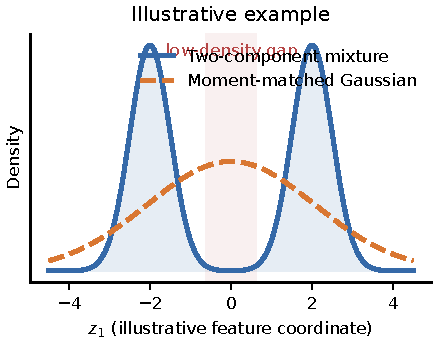
\includegraphics[width=\columnwidth]{figures/misfp_multimodality.pdf}
\caption{\textbf{Illustrative example} generated from the specified mixture $0.5\mathcal N((-2,0),\mathrm{diag}(0.25,0.49))+0.5\mathcal N((2,0),\mathrm{diag}(0.25,0.49))$. A moment-matched diagonal Gaussian preserves the plotted marginal moments but allocates density between modes. This is synthetic explanation, not a learned result.}
\label{fig:illustration}
\end{figure}
